\documentclass[11pt,a4paper,titlepage]{article}
\usepackage[utf8]{inputenc}
\usepackage[english]{babel}
\usepackage{lipsum}
\usepackage[a4paper, top=2.5cm, bottom=2.5cm, left=2.2cm, right=2.2cm]{geometry}
\usepackage{csquotes}


\usepackage{amsmath, amssymb, amsfonts, amsthm, fouriernc, mathtools}
% mathtools for: Aboxed (put box on last equation in align envirenment)
\usepackage{microtype} %improves the spacing between words and letters

\usepackage{graphicx}
\graphicspath{ {./pics/} {./eps/}}
\usepackage{epsfig}
\usepackage{epstopdf}


%%%%%%%%%%%%%%%%%%%%%%%%%%%%%%%%%%%%%%%%%%%%%%%%%%
%% COLOR DEFINITIONS
%%%%%%%%%%%%%%%%%%%%%%%%%%%%%%%%%%%%%%%%%%%%%%%%%%
\usepackage[svgnames]{xcolor} % Enabling mixing colors and color's call by 'svgnames'
%%%%%%%%%%%%%%%%%%%%%%%%%%%%%%%%%%%%%%%%%%%%%%%%%%
\definecolor{MyColor1}{rgb}{0.2,0.4,0.6} %mix personal color
\newcommand{\textb}{\color{Black} \usefont{OT1}{lmss}{m}{n}}
\newcommand{\blue}{\color{MyColor1} \usefont{OT1}{lmss}{m}{n}}
\newcommand{\blueb}{\color{MyColor1} \usefont{OT1}{lmss}{b}{n}}
\newcommand{\red}{\color{LightCoral} \usefont{OT1}{lmss}{m}{n}}
\newcommand{\green}{\color{Turquoise} \usefont{OT1}{lmss}{m}{n}}
%%%%%%%%%%%%%%%%%%%%%%%%%%%%%%%%%%%%%%%%%%%%%%%%%%




%%%%%%%%%%%%%%%%%%%%%%%%%%%%%%%%%%%%%%%%%%%%%%%%%%
%% FONTS AND COLORS
%%%%%%%%%%%%%%%%%%%%%%%%%%%%%%%%%%%%%%%%%%%%%%%%%%
%    SECTIONS
%%%%%%%%%%%%%%%%%%%%%%%%%%%%%%%%%%%%%%%%%%%%%%%%%%
\usepackage{titlesec}
\usepackage{sectsty}
%%%%%%%%%%%%%%%%%%%%%%%%
%set section/subsections HEADINGS font and color
\sectionfont{\color{MyColor1}}  % sets colour of sections
\subsectionfont{\color{MyColor1}}  % sets colour of sections

%set section enumerator to arabic number (see footnotes markings alternatives)
\renewcommand\thesection{\arabic{section}.} %define sections numbering
\renewcommand\thesubsection{\thesection\arabic{subsection}} %subsec.num.

%define new section style
\newcommand{\mysection}{
\titleformat{\section} [runin] {\usefont{OT1}{lmss}{b}{n}\color{MyColor1}} 
{\thesection} {3pt} {} } 

%%%%%%%%%%%%%%%%%%%%%%%%%%%%%%%%%%%%%%%%%%%%%%%%%%
%		CAPTIONS
%%%%%%%%%%%%%%%%%%%%%%%%%%%%%%%%%%%%%%%%%%%%%%%%%%
\usepackage{caption}
\usepackage{subcaption}
%%%%%%%%%%%%%%%%%%%%%%%%
\captionsetup[figure]{labelfont={color=Turquoise}}

%%%%%%%%%%%%%%%%%%%%%%%%%%%%%%%%%%%%%%%%%%%%%%%%%%
%		!!!EQUATION (ARRAY) --> USING ALIGN INSTEAD
%%%%%%%%%%%%%%%%%%%%%%%%%%%%%%%%%%%%%%%%%%%%%%%%%%
%using amsmath package to redefine eq. numeration (1.1, 1.2, ...) 
%%%%%%%%%%%%%%%%%%%%%%%%
\renewcommand{\theequation}{\thesection\arabic{equation}}

%set box background to grey in align environment 
\usepackage{etoolbox}% http://ctan.org/pkg/etoolbox
\makeatletter
\patchcmd{\@Aboxed}{\boxed{#1#2}}{\colorbox{black!15}{$#1#2$}}{}{}%
\patchcmd{\@boxed}{\boxed{#1#2}}{\colorbox{black!15}{$#1#2$}}{}{}%
\makeatother
%%%%%%%%%%%%%%%%%%%%%%%%%%%%%%%%%%%%%%%%%%%%%%%%%%




%%%%%%%%%%%%%%%%%%%%%%%%%%%%%%%%%%%%%%%%%%%%%%%%%%
%% DESIGN CIRCUITS
%%%%%%%%%%%%%%%%%%%%%%%%%%%%%%%%%%%%%%%%%%%%%%%%%%
\usepackage[siunitx, american, smartlabels, cute inductors, europeanvoltages]{circuitikz}


\makeatletter
\let\reftagform@=\tagform@
\def\tagform@#1{\maketag@@@{(\ignorespaces\textcolor{red}{#1}\unskip\@@italiccorr)}}
\renewcommand{\eqref}[1]{\textup{\reftagform@{\ref{#1}}}}
\makeatother
\usepackage{hyperref}
\hypersetup{colorlinks=true}

\title{ CS $215$ 

\blueb Homework $1$}
\author{
  Omkar Shirpure\\
  \texttt{22B0910}
  \and
  Krish Rakholiya\\
  \texttt{22B0927}
}
\date{}
%%%%%%%%%%%%%%%%%%%%%%%%%%%%%%%%%%%%%%%%%%%%%%%%%%



\begin{document}
\maketitle

\section{Question 1 : }{
\subsection{}{
The probability of the every person picking their own notebook is (for the first person to get his own notebook is $\frac{1}{n}$, for the second person $\frac{1}{n-1}$ and so on... ) 

So their overall probability is
$$P = \frac{1}{n}*\frac{1}{n-1} ... \frac{1}{2}*\frac{1}{1}$$
Hence,
$$P = \frac{1}{n!}$$
}

\subsection{}{
The probability of getting the correct notebooks for the first m(<n) people could be calculated by same method. W.K.T. (for the first person to get his own notebook is $\frac{1}{n}$, for the second person $\frac{1}{n-1}$ up to $m$th person $\frac{1}{n-m+1}$)

\vspace{0.2cm}
The overall probability will be
$$P = (\frac{1}{n})(\frac{1}{n-1})(\frac{1}{n-2})...(\frac{1}{n-m+1})$$
$$P = \frac{(n-m)!}{n!}$$
$$P = \frac{1}{m!}\binom{n}{m}^{-1}$$
}

\subsection{}{
This is conceptually same as the previous one, where just the set of $m$ changes from first to last. First person will have $m$ choices from $n$ books and the second one will have $m-1$ choice from $n-1$ books and so on.
Hence,
$$P = \frac{m}{(n)}\frac{m-1}{(n-1)}\frac{m-2}{(n-2)}...\frac{1}{(n-m+1)}$$
$$P = \binom{n}{m}^{-1}$$
}

\subsection{}{
The probability of getting clean books for first $m$ persons is 
$$P = (1-p)^m$$
since the probability of book being clean is independent of any other factors.
}

\subsection{}{
Since it is given that first $m$ persons pick up clean books (with probability (1-p)) and rest of the $(n-m)$ people pick up unclean books (with probability p).
The total probability is 
$$P = \binom{n}{m}(1-p)^m(p)^{n-m}$$
}
\newpage







\section{Question 2 : }{
We are given n distinct values $x_i$ with their mean $\mu$ and standard deviation $\sigma$ and to prove 
$$|x_i-\mu| \leq \sigma \sqrt{n-1}$$
Since we defined the variance as 
$$\sigma^2 = \frac{\Sigma(x_i - \mu)^2}{n-1}$$
From the equation to prove, squaring on both sides and expanding, it gives,
$$(x_i - \mu)^2 \leq \sigma^2(n-1) $$
$$x_i^2 -2x_i\mu + \mu^2 \leq \sigma^2(n-1)$$
Taking expectation of both sides,
$$E(x_i^2) - 2\mu E(x_i) + \mu^2 \leq $$
$$E(x_i^2) - \mu^2 \leq \sigma^2(n-1)$$
Since, Var $ = E(x_i^2) - \mu^2$, substituting we get,
$${var} \leq \sigma^2(n-1)$$
$${var} \leq {var}(n-1)$$

And since, variance is always non-negative, this inequality holds true. And hence the inequality $|x_i-\mu| \leq \sigma \sqrt{n-1}$ holds true for all individual $x_i$. \\

Coming to comparison with Chebyshev's Inequality as $n$ increases, the above becomes a more stronger statement compared to Chebyshev's Inequality. Chebyshev's Inequality in general being just the probabilistic bound for all distributions, but the above inequality gives a direct relation between all the individual data points, and other details such as mean, standard deviation, etc.And as $n$ increases, the proven inequality becomes more accurate and informative for this specific data set as compared to Chebyshev's inequality.
}
\newpage






\section{Question 3 : }{
We are given that $\varepsilon > 0$ and two values $Q_1$ and $Q_2$ alongside the events $F$ and $E$ , ie.
\[ F : |Q_1 + Q_2| >\varepsilon \]
\[ E : |Q_1| + |Q_2| > \varepsilon \]
$E_1$ and $E_2$ be the events $|Q_1| > \varepsilon/2$  and  $|Q2| > \varepsilon/2$ respectively .
\\\\Now, By simple Triangle law of inequality, 
\[ \varepsilon < |Q_1 + Q_2| < |Q_1|+|Q_2|\]
Thus the values of $Q_1$ and $Q_2$ satisfying $F$ will also satisfy $E$. 
In other words \, $ F \subset  E$ . So,
\\ 
\begin{equation}{
P(E) \geqslant P(F) 
}
\end{equation}
Now,
$$P(E) \, \, \, or \, \, \, P(|Q_1|+|Q_2|> \varepsilon) \leqslant P(Either \; of \; Q \; has\; the\; absolute\; value > \varepsilon/2) $$
$$=P(|Q_1| > \varepsilon/2 \; \cup \;|Q_2| > \varepsilon/2)$$
$$ = \; P(|Q_1| > \varepsilon/2) \; + \; P(|Q_2| > \varepsilon/2) \; - \; P(|Q_1| > \varepsilon/2)*P(|Q_2| > \varepsilon/2)$$
$$ = \; P(E_1) \; + \; P(E_2) \; - \; P(E_1)*P(E_2)$$
$$ \leqslant P(E_1) \; +\; P(E_2) $$
Thus ,
\begin{equation}
    P(E) \; \leqslant \; P(E_1) \;+ \; P(E_2)
\end{equation}
Thus , combining eq. 3.1 and 3.2 , We get
$$P(F) \; \leqslant \; P(E) \leqslant  \; P(E_1) \;+ \; P(E_2)$$
Finally ,
$$P(F) \; \leqslant  \; P(E_1) \;+ \; P(E_2)$$
$\therefore$ \; Hence, Proved .
}
\newpage







\section{Question 4 : }{
We are given 2 non-negative random variable $Q_1$ and $Q_2$ alongside $q_1$and $q_2$, both are non-negative.
\\ Given , \; $P(Q_1 \; < \; q_1) \; \geqslant \; 1 \;-\; p_1$ \; and \; $P(Q_2 \; < \; q_2) \; \geqslant \; 1 \;-\; p_2$.
It can be written that 
$$P(Q_1*Q_2 \; < \; q_1*q_2) \; = \; P(Q_1 \; < \; q_1 \; \cap \; Q_2 \; < \; q_2) \; + \; P(Q_1 \; > \; q_1 \; but \; Q_1*Q_2 \; < \; q_1*q_2)\; + \; P(Q_2 \; > \; q_2 \; but \; Q_1*Q_2 \; < \; q_1*q_2)$$
Or in other words, 
$$P(Q_1*Q_2 \; < \; q_1*q_2) \; = \; P(Q_1 \; < \; q_1 \; \cap \; Q_2 \; < \; q_2) \; + \; P_1\; + \; P_2$$
where $P_1$ and $P_2$ are the respective probabilities from the above equation.\\
So , We can write that
$$P(Q_1*Q_2 \; < \; q_1*q_2) \; \geqslant \; P(Q_1 \; < \; q_1 \; \cap \; Q_2 \; < \; q_2) $$
As selection of $Q_1$ and $Q_2$ are independent, So
$$P(Q_1*Q_2 \; < \; q_1*q_2) \; \geqslant \; P(Q_1 \; < \; q_1)*P( Q_2 \; < \; q_2) $$
$$\geqslant \; (1-p_1)\; * \;(1-p_2)$$
$$= \; 1\; - \; p_1 \; -\; p_2\; + \; p_1*p_2$$
$$\geqslant 1\; - \; p_1 \; -\; p_2$$
$\therefore$ \; Hence ,Proved that
$$P(Q_1*Q_2 \; < \; q_1*q_2) \; \geqslant 1\; - \; p_1 \; -\; p_2$$
}
\newpage






\section{Question 5 : }{
Given , $P(C_i)$ be the probability of having a car behind the door $i\; ( i=1\;,2\;,3)$ = 1/3 .\\
$Z_i$ be the event that the contestant chose door $i\; ( i=\;1,\;2,\;3)$ \\
$H_i$ be the event that the host opened door $i\; ( i=\;1,\;2,\;3)$.
\subsection{}{
$$P(C_i\; / \; Z_i)\;=\frac{P(C_i\; \cap \; Z_i)}{P( Z_i)}$$
As the event of choosing a door and of having a car behind a door are independent , So
$$P(C_i\; / \; Z_i)\;=\frac{P(C_i)*P(Z_i)}{P(Z_i)}$$
$$=P(C_i)$$
$$=\frac{1}{3}$$
for all i \; =\; 1,\;2,\;3
}
\subsection{}{
$$P(H_3/C_i\;,\; Z_1)=\; \frac{P(H_3\;\cap\;(C_i\;,\; Z_1))}{P(C_i\;,\; Z_1)}$$
\begin{itemize}
    \item Now , for i=1\\
    The expression $P(H_3/C_1\;,\; Z_1)$ asks the probability that the host opens door 3 given that the person opens the door 1 and the car is also in door 1.\\
    The person opening the door 1 and the car is also in door 1 leads to 2 cases , ie. the host opens either door 2 or the door 3 .\\
    As both the event has equally likely to happen.\\
    So, the Probability of him opening the door 3 will turn out to be $\frac{1}{2}$ 
    $$P(H_3/C_1\;,\; Z_1)\;=\;\frac{1}{2}$$
    \item Now , for i=2\\
    The expression $P(H_3|C_2\;,\; Z_1)$ asks the probability that the host opens door 3 given that the person opens the door 1 and the car is also in door 2.\\ 
    The person opening the door 1 and the car is in door 2 leads to only 1 case , ie. the host will open door 3 , as he knows that door 2 has the car in it ,thus can't open it .\\
    So , the Probability of the host opening the door 3 is 1(the only possibility).
    $$P(H_3/C_2\;,\; Z_1)\;=\;1$$
    \item Now , for i=3\\
    The expression $P(H_3|C_3\;,\; Z_1)$ asks the probability that the host opens door 3 given that the person opens the door 1 and the car is also in door 3.\\ 
    The person opening the door 1 and the car is in door 3 leads to only 1 case , ie. the host will open door 2 , as he knows that door 3 has the car in it ,thus can't open it .\\
    So , the Probability of the host opening the door 3 is 0 (not possibility).
    $$P(H_3/C_3\;,\; Z_1)\;=\;0$$
\end{itemize}
}
\newpage
\subsection{}{
The conditional probability of winning by switching is $P(C_2/H_3,\; Z_1)$. Also
$$P(C_2/H_3,\; Z_1)\;=\; \frac{P(H_3/C_2, \;Z_1)P(C_2,\; Z_1)}{P(H_3,\; Z_1)}$$
As we already know , $P(H_3/C_2\;,\; Z_1)\;=\;1$ \;So,
$$P(C_2/H_3,\; Z_1)\;=\; \frac{1\;*\;P(C_2,\; Z_1)}{P(H_3,\; Z_1)}$$
$$=\; \frac{P(C_2\;\cap\; Z_1)}{P(H_3\;\cap\; Z_1)}$$
$$=\; \frac{P(C_2)*P( Z_1)}{P(H_3 /\;Z_1)*P(Z_1)}$$
$$=\; \frac{P(C_2)}{P(H_3 /\;Z_1)}$$
Now to compute the probability $P(H_3 /\;Z_1)$ which is the Probability that the host will open door 3 if the contestant chooses door1  , \\
$$P(H_3 /\;Z_1) \; =\;P(C_1)P(H_3/C_1\;,\; Z_1)\;+\;P(C_2)P(H_3/C_2\;,\; Z_1)\;+\;P(C_3)P(H_3/C_3\;,\; Z_1) $$
As all the RHS values are already computed,
$$P(H_3 /\;Z_1) \; =\;\frac{1}{3}*\frac{1}{2}\;+\;\frac{1}{3}*1\;+\;\frac{1}{3}*0\;=\;\frac{1}{2}$$
So, finally
$$P(C_2/H_3,\; Z_1)\;=\;\frac{P(C_2)}{P(H_3 /\;Z_1)} \;=\; \frac{1/3}{1/2} $$
$$P(C_2/H_3,\; Z_1)\;=\;\frac{2}{3}$$
}

\subsection{}{
The conditional probability of winning by switching is $P(C_1/H_3,\; Z_1)$. Also
$$P(C_1/H_3,\; Z_1)\;=\; \frac{P(H_3/C_1, \;Z_1)P(C_1,\; Z_1)}{P(H_3,\; Z_1)}$$
As we already know , $P(H_3/C_1\;,\; Z_1)\;=\;1/2$ \;So,
$$P(C_1/H_3,\; Z_1)\;=\; \frac{1/2\;*\;P(C_1,\; Z_1)}{P(H_3,\; Z_1)}$$
$$=\; \frac{P(C_1\;\cap\; Z_1)}{2*P(H_3\;\cap\; Z_1)}$$
$$=\; \frac{P(C_1)*P( Z_1)}{2*P(H_3 /\;Z_1)*P(Z_1)}$$
$$=\; \frac{P(C_1)}{2*P(H_3 /\;Z_1)}$$
As we already know the value of $P(H_3 /\;Z_1)$ which is $\frac{1}{2}$
So, 
$$P(C_1/H_3,\; Z_1)\;=\;\frac{P(C_1)}{2*P(H_3 /\;Z_1)} \;=\; \frac{1/3}{2*1/2} $$
$$P(C_1/H_3,\; Z_1)\;=\;\frac{2}{3}$$
}
\newpage
\subsection{}{
Looking at the above parts of this question , as the probability of winning by switching (part 5.3) = $\frac{2}{3}$ is greater than the probability of winning by not switching (part 5.4) =$\frac{1}{3}$.\\
So , We can conclude that switching the door here is more beneficial than remaining on the previously selected door.
}

\subsection{}{
Considering that the person chose door 1 .Then,
\begin{itemize}
    \item Switching the door (to door 2)
    $$P(C_2/H_3,\; Z_1)\;=\; \frac{P(H_3/C_2, \;Z_1)P(C_2,\; Z_1)}{P(H_3,\; Z_1)}$$
    As there are 2 remaining door , so opening either of them will be equally likely and irrespective of car in any of the door and thus , equal to 1/2. \\
    So , $P(H_3/C_2, \;Z_1) =\; P(H_3/\;Z_1)\; = 1/2$
    $$P(C_2/H_3,\; Z_1)\;=\; \frac{1/2*P(C_2,\; Z_1)}{P(H_3,\; Z_1)}$$
    $$=\; \frac{1/2*P(C_2\cap\; Z_1)}{P(H_3\cap\; Z_1)}$$
    $$=\; \frac{1/2*P(C_2)*\;P( Z_1)}{P(H_3/Z_1)\;*\; P(Z_1)}$$
    $$=\;\frac{P(C_2)}{2*P(H_3/Z_1)}$$
    $$=\;\frac{1/3}{2*1/2} \;= \;\frac{1}{3}$$
    
    \item Switching the door (to door 3)
    $$P(C_3/H_3,\; Z_1)\;=\; \frac{P(H_3/C_3, \;Z_1)P(C_3,\; Z_1)}{P(H_3,\; Z_1)}$$
    As there are 2 remaining door , so opening either of them will be equally likely and irrespective of car in any of the door and thus , equal to 1/2. \\
    So , $P(H_3/C_3, \;Z_1) =\; P(H_3/\;Z_1)\; = 1/2$
    $$P(C_3/H_3,\; Z_1)\;=\; \frac{1/2*P(C_3,\; Z_1)}{P(H_3,\; Z_1)}$$
    $$=\; \frac{1/2*P(C_3\cap\; Z_1)}{P(H_3\cap\; Z_1)}$$
    $$=\; \frac{1/2*P(C_3)*\;P( Z_1)}{P(H_3/Z_1)\;*\; P(Z_1)}$$
    $$=\;\frac{P(C_3)}{2*P(H_3/Z_1)}$$
    $$=\;\frac{1/3}{2*1/2} \;= \;\frac{1}{3}$$

    \item Not switching the door (remaining in door 1)
    $$P(C_1/H_3,\; Z_1)\;=\; \frac{P(H_3/C_1, \;Z_1)P(C_1,\; Z_1)}{P(H_3,\; Z_1)}$$
    As there are 2 remaining door , so opening either of them will be equally likely and irrespective of car in any of the door and thus , equal to 1/2. \\
    So , $P(H_3/C_1, \;Z_1) =\; P(H_3/\;Z_1)\; = 1/2$
    $$P(C_1/H_3,\; Z_1)\;=\; \frac{1/2*P(C_1,\; Z_1)}{P(H_3,\; Z_1)}$$
    $$=\; \frac{1/2*P(C_1\cap\; Z_1)}{P(H_3\cap\; Z_1)}$$
    $$=\; \frac{1/2*P(C_1)*\;P( Z_1)}{P(H_3/Z_1)\;*\; P(Z_1)}$$
    $$=\;\frac{P(C_1)}{2*P(H_3/Z_1)}$$
    $$=\;\frac{1/3}{2*1/2} \;= \;\frac{1}{3}$$   
\end{itemize}
Thus ,We can conclude that in this case switching will have no further benefit for the contestant.
\\
Winning in both the cases is equally likely.
}






}
\newpage






\section{Question 6 : }{
\textit{The code and plots for this question has been included in the folder.} \\
\begin{itemize}
    \item at $f = 30\%$
    \begin{itemize}
        \item The RMS error of moving median filtering is $15.186$.
        \item The RMS error of moving mean filtering is $58.9177$.
        \item The RMS error of moving quartile filtering is $0.015119$.
    \end{itemize}
    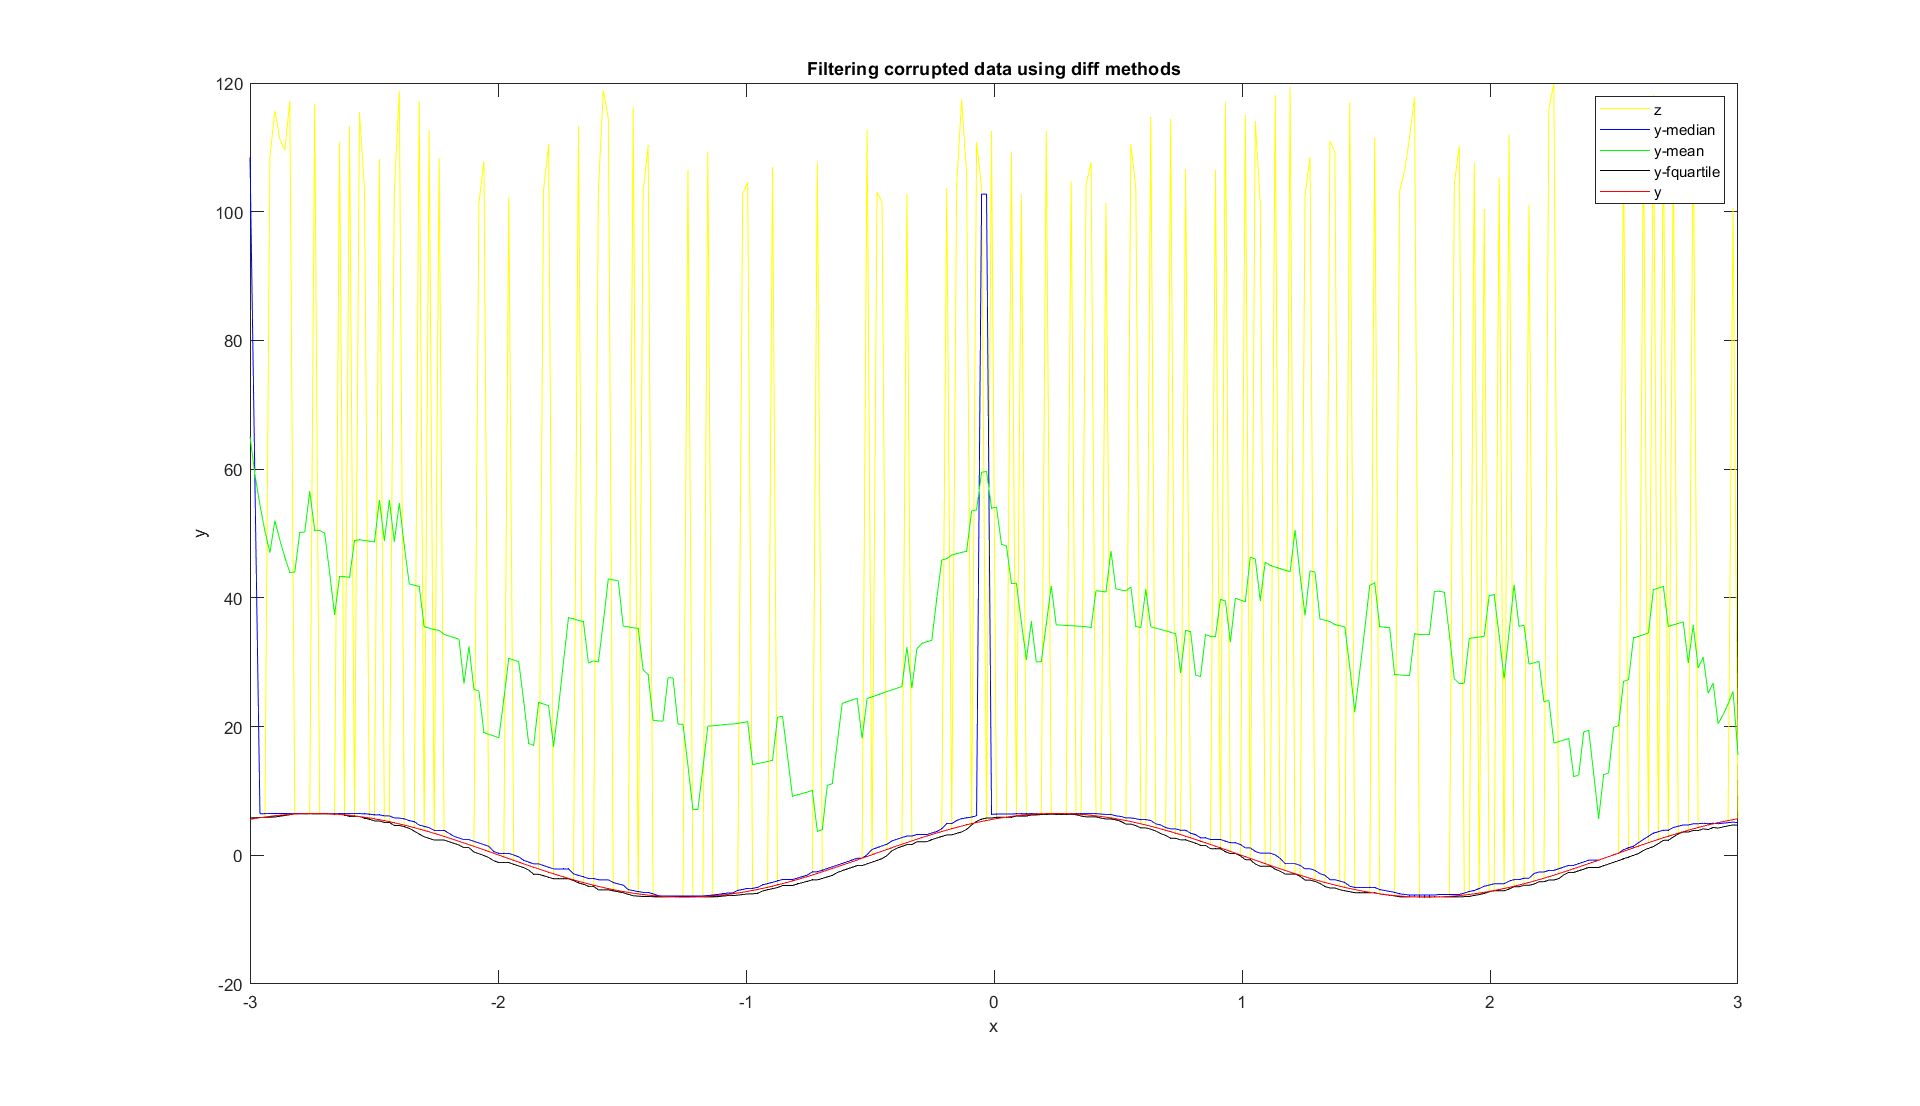
\includegraphics[width=15cm, height=8cm]{images/q6_1.png}
    \item at $f = 60\%$
    \begin{itemize}
        \item The RMS error of moving median filtering is $420.5754$.
        \item The RMS error of moving mean filtering is $215.2678$.
        \item The RMS error of moving quartile filtering is $45.1039$.
    \end{itemize}
    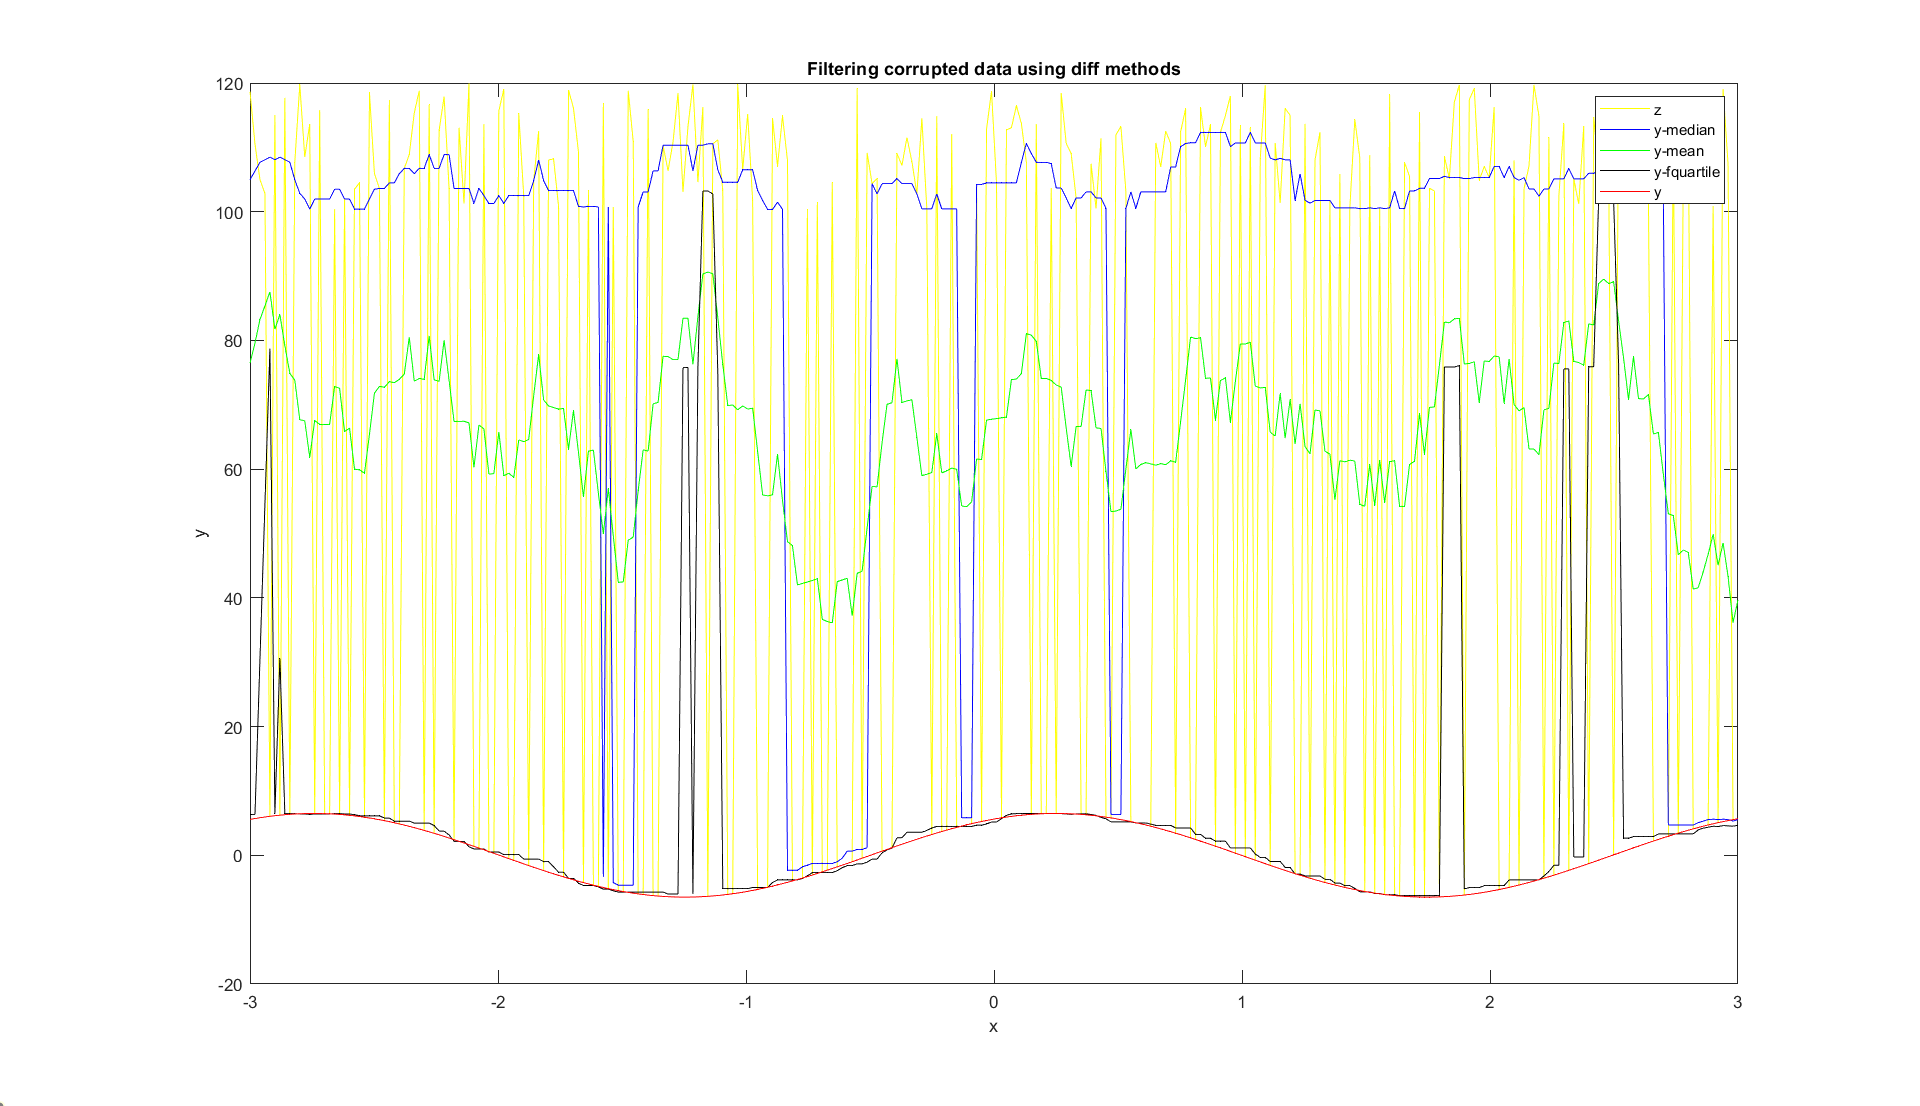
\includegraphics[width=15cm, height=9cm]{images/q6_2.png}
\end{itemize}
The moving quartile method seems to be more accurate and produces better results in RMS error. \\

The noise reduction using \emph{mean method} is least efficient since mean is more sensitive to larger noise values. The \emph{median method} in this case being more accurate since we consider the middle element by sequence, it is robust to the larger noise values. But may be inefficient in the cases of extreme noisy conditions (eg. $f = 60\%$).

And in the end, the \emph{quartile method}, which focuses on the middle 50\% of the data, is most robust against noise and outliers.

}
\newpage






\section{Question 7 :}{
\begin{itemize}
    \item Updating the value of the bin \\
    
    When we receive the new data value to be added into A, that new value or the data-point will fall into its corresponding bin by finding the range into which the value belongs to. And then increment the value or count of that bin by $1$. \\
\end{itemize}


Recalculating the values for the updated data consisted in the A is computationally inefficient. Hence, defining functions to recalculate the data in a smart way becomes necessary. Also in histogram's case, some times the number of bins might be much smaller than the total number of data points, updating the histogram is generally more efficient than recomputing the entire histogram from scratch. This is particularly important when dealing with large data-sets.
}

\end{document}